\chapter{Intermediate Models of STDP}
\label{chap:ModelIntermediate_STDP}

This type of models requires details description of the neuron:
These models require explicit modelling of 
\begin{enumerate}
  \item internal voltage (neuronal potential)
  
  \item back-propagating AP (bAP) - Sect.\ref{sec:bAP}
  
  \item individual ion channels
  
%  \item chemical networks
  
  \item description of synaptic plasticity due to mechanism such as AMPAR
  trafficking or AMPAR phosphorylation
\end{enumerate}



\section{Karmarka-Buounomano (2002) - role of $\Ca$}
\label{sec:Karmarka-Buounomano-2002}


This model examine the role of postsynaptic $\Ca$ through NMDAR:
\begin{itemize}
  \item moderate increase $[\Ca]$ induce LTD
  \item large increase ${\Ca}$ induce LTD
\end{itemize}
Specifically, it is unclear why an NMDAR-based model would produce little or no
LTD at long negative interspike intervals (ISIs) and maximal LTD at short ones.


This study captures postsynaptic $\Ca$ influx dynamics and the associativity of
the NMDA receptors. A few models have been tested.
Their results predict that a second coincidence detector
is necessary to account for the temporal properties of STDP.

\subsection{Model 1}

The first of these models is based on the NMDAR as an associative molecule
coupled with the assumptions of the standard model.
It is assumed that the increase in $\Ca$, regardless of the source, above the
baseline account for both LTD and LTP.

$\Ca$ influx through 2 pathways: $V_m$-gated $\Ca$ channels (VGCC) and NMDAR,
which is modeled as
\begin{itemize}
  \item VGCC: sigmoidal function dependent on the membrane voltage, with $\tau
  = 15$ ms decay time constant, and driving force of $(v-140)$
  
\begin{equation}
\frac{d[\Ca_{VGCC}]}{dt} = \left[ k_1(V_m-140)\sigma(V_m) \right] -
\frac{[\Ca_{VGCC}]}{\tau}
\end{equation}  
with $k_1 = -0.023$, and the $V_m$-dependent channel kinetics
$\sigma(V_m) = \frac{1}{1+\exp(-V_m+0.1)}$.

  \item NMDAR: the gating of NMDAR is a function of $V_m$, the presence of
  bound glutamate, and the blocking of $\Mg$.
  
  The blocking of $\Mg$ is modelled as a sigmoidal $V_m$-dependent function:
  \begin{equation}
  B(V_m) = 	\frac{1}{1+\exp(0.0868 (-V_m-10))}
  \end{equation}
  approximated from experimental data (Bekkers and Stevens 1993).
  
  The change in $\Ca$ entering via NMDAR is
\begin{equation}
\frac{d[\Ca_{NMDAR}]}{dt} = \left(  -0.008 (V_m-140) \left[
B(v)\frac{R_{NMDAR}}{k_2} \right] \right) - \frac{[\Ca_{NMDAR}]}{\tau}
\end{equation}
There are 2 dissociation constants: $\beta = 0.075, k_2 = 0.6178$ and 
$\beta = 0.025, k_2 = 0.6792$.

The each ISI, the maximum of this sum $[\Ca_{VGCC}]+[\Ca_{NMDAR}]$, and a
plot of the peak $[\Ca]$ as a function if ISI, and the value was used to
calculate plasticity.
The plasticity $P$ as a function of $[\Ca]_\peak$
\begin{equation}
P([\Ca]_\peak) = 2.8 \left[ \frac{1}{1+\exp(4(-[\Ca]_peak - k_3))}  \right]
 - 2 \left[ \frac{1}{1+ \exp(12(-[\Ca]_\peak - k_4))} \right] + 0.7858
\end{equation}=
with $\beta = 0.075$, $k_3 = 0.2118$, $k_4 = 0.7128$, and for  $\beta= 0.025$,
$k_3 = 0.4534$, $k_4 = 0.9314.$.

QUESTION: \textcolor{red}{Why there are two sets of values here?}

\end{itemize}

\subsection{Model 2}

% In the previous model, the two $\Ca$ sources act independently, i.e. the influx
% of $\Ca$ in one source does not impact the influx of $\Ca$ in the other source.
In this model, a second associative mechanism is added:
It is assumed two $\Ca$ sources act independently, i.e. the influx
of $\Ca$ via VGCC involve in LTD; while the influx
of $\Ca$ via NMDAR involve in LTP.
 
 
 The second involves the NMDAR and an additional coincidence
detector that is primarily responsible for the timing sensitivity
of LTD.

\subsection{Numerical analysis}

A presynaptic and postsynaptic neuron model were simulated.
Each cell was modeled as an integrate-and-fire unit
(Sect.\ref{sec:leaky_integrate-and-fire_model}):
$E_\leak = -60$ mV, spike threshold $V_{th} = -40$ mV, the reset potential
$V_\reset = -56$ mV (after the spike). 

All simulations were conducted using program NEURON.

\section{Shouval etl a. (2002)}
\label{sec:Shouval-2002}

\subsection{Assumption}

\citep{shouval2002} constructed a model 
based on 3 assumptions
\begin{enumerate}
  \item $[\Ca]$ is the primary signal for synaptic plasticity (LTP, LTD)
  
  \item The dominant source of $\Ca$ flux is the influx via NMDAR
  (Sect.\ref{sec:NMDAR}) 
  
  (\textcolor{red}{How about the role of $\Ca$ release via IP3R from ER})
  
  \item dendritic bAP contributing to STDP (Sect.\ref{sec:STDP}) has a slow
  'after-depolarizing' tail components (Sect.\ref{sec:bAP})
  
  They reasoned that if bAP is short, e.g. 3ms, the effect of removing
  $\Mg$-block is short, and thus its effect on increasing $\Ca$ influx via NMDAR
  is little. So, they proposed a wider tail as the result of the sum of two
  exponential components.
  
  
  \item As AMPAR is activated first under presynaptic neurotransmitter
  release, AMPAR activation is modelled as a synaptic weight $W_j$
  
  \item The resting $V_\rest = -65$ (mV), slightly lower than found in most
  hippocampal cells and slightly above the value for most cells in neocortex.
  
  \item Only EPSP generated by AMPAR current and bAP contributes to the
  postsynaptic $V_m$. It is assumed that NMDAR plays no contribution to $V_m$.
  
  
  \item The arrival time of the bAP is assumed 2-ms delay, so the forms of
  depolarization add linearly. 
    
\end{enumerate}

% \begin{enumerate}
%   \item $\Ca$ is the primary signal for synaptic plasticity
%   
%   \item dominant source of $\Ca$ influx is via NMDAR (Sect.\ref{sec:NMDAR})
%   
%   \item dendritic backpropagating AP contributing to STDP (Sect.\ref{sec:STDP})
%   has a slow 'after-depolarizing' tail component
%   (Sect.\ref{sec:back-propagating_AP})
% \end{enumerate}


\subsection{Model }

At synapse $j$, the synapse strength is
\begin{equation}
\dot{W_j} =\frac{dW_j}{dt} = \eta \times \Omega\left( [\Ca]_j \right)
\end{equation}
with $\eta $ is learning rate.
The $\Omega(\cdot)$ function receives different values (in the range [0,1])
depending on the value of $[\Ca]$, as shown in Fig.\ref{fig:Shouval2012_omega_eta} (A)
\begin{itemize}
  \item $[\Ca] < \theta_d$ : no modification occurs
  
  \item $\theta_d < [\Ca] < \theta_p$: LTD (i.e. $W_j$ is depressed)
  
  \item $\theta_p < [\Ca]$: LTP (i.e. $W_j$ is potentiated)
\end{itemize}
\def\sig{{\text{sig}}}
\begin{equation}
\Omega = 0.25 + \sig \left( [\Ca] - \alpha_2, \beta_2 \right) - 
         0.25 \sig \left( [\Ca]-\alpha_1, \beta_1 \right)
\end{equation}
with $\sig(x,\beta) = \frac{\exp(\beta x)}{1 + \exp(\beta x)}$
(Sect.\ref{sec:sigmoidal-relation})

\begin{figure}[htb]
  \centerline{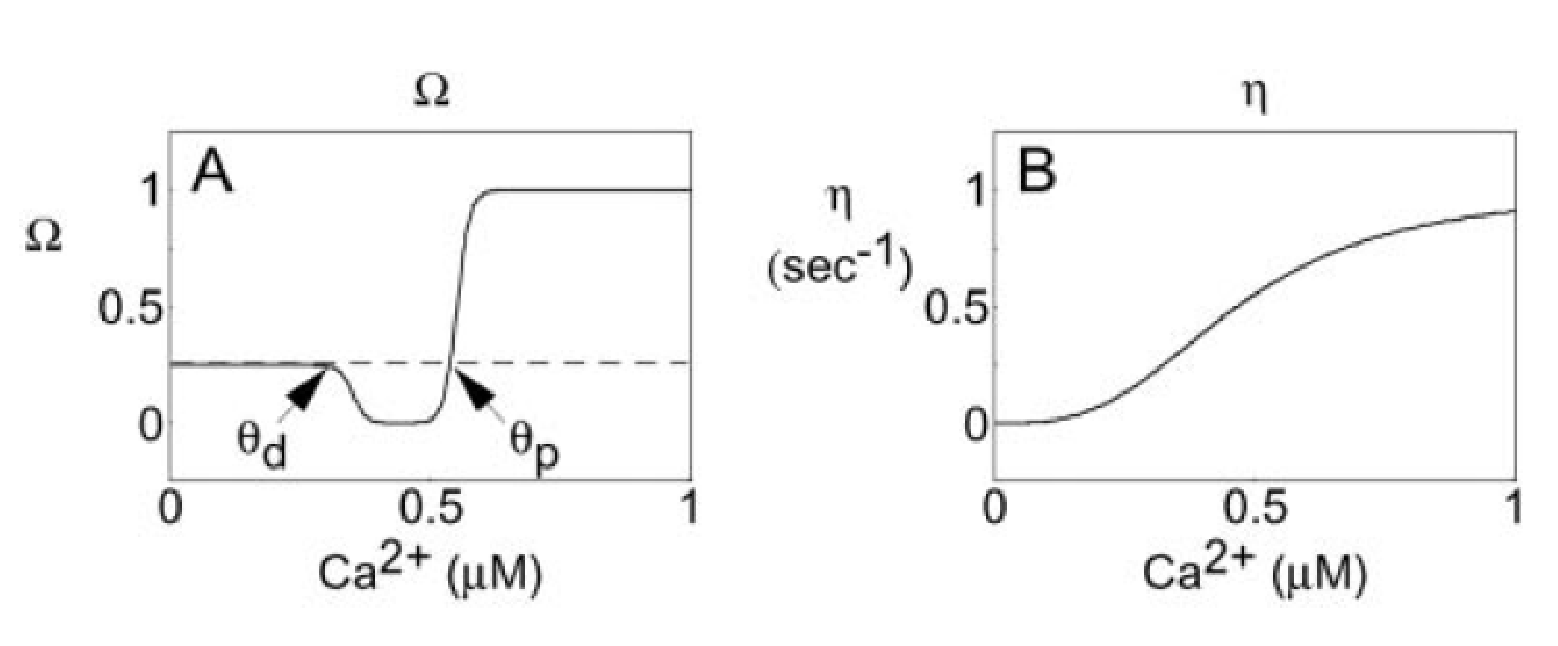
\includegraphics[height=5cm]{./images/Shouval2012_omega_eta.eps}}
  \caption{(A) Omega function, (B) learning
  rate $\eta$}\label{fig:Shouval2012_omega_eta}
\end{figure}

\textcolor{red}{Constraints}: to avoid $W_j$ increases/decreases indefinitely,
there are two approaches
\begin{enumerate}
  \item set a lower and upper boundary
  \item add a weight decay term
  
\begin{equation}
\dot{W_j} =\frac{dW_j}{dt} = \eta \times \left(\Omega\left( [\Ca]_j \right) -
\lambda W_j \right) 
\end{equation}
with $\lambda$ is the decay constant. 
This equation has a fixed point for a given calcium level and does not usually
converge to the upper or lower saturation bounds.

An unwanted behavior of using the decay term is that the synaptic weights
rapidly converge back to their initial values when calcium returns to the basal
level. In addition, the constant learning rate for potentiation and depression
can lead to unwanted oscillations in synaptic weight.

  \item To slow down the change in the synaptic weight, they proposed a dynamic
  learning rate which is a function of $[\Ca]_i$
  
\begin{equation}
\dot{W_j} =\frac{dW_j}{dt} = \eta([\Ca]_j) \times \left(\Omega\left( [\Ca]_j
\right) - W_j \right)
\end{equation}
with $\eta(\cdot)$ is assumed a monotonically increase function of $[\Ca]_j$ (a
sigmoidal function), as shown in Fig.\ref{fig:Shouval2012_omega_eta}(B); and
$\lambda=1$ is chosen without the loss of generality.
  
 \textcolor{red}{NOTE}: The learning rate $\eta$ is inversely proportional to
 the learning time constant $\tau$.
\begin{equation}
\eta = \frac{1}{\tau}
\end{equation}

with 
\begin{equation}
\tau = \frac{P_1} {P_2 + ([\Ca])^{P_3}} + P_4
\end{equation}
with $P_1 = 0.1$ (sec), $P_2 = P_1 \times 10^4$ (sec), $P_3 = 3$, and 
$P_4 = 1$ (sec).


\end{enumerate}

\textcolor{red}{\bf NMDAR $\Ca$ current} is given in Sect.\ref{sec:NMDAR-Shouval
(2002)}.


\textcolor{red}{\bf $\Ca$ dynamics}:
\begin{equation}
\frac{d[\Ca]_i}{dt} = I_\NMDA(t) - \frac{1}{\tau_\ca} [\Ca]_i
\end{equation}
which is assumed to be removed out of the spine head at a rate of time constant
$\tau_\ca = 50$ (ms). This is an non-physiological value chosen as
an intermediate value between the different published results [see 21, 25].


\textcolor{red}{\bf bAP}: The bAP is modeled as the sum of two exponential
terms: a fast term ($\tau_f^\bAP=3$ms) and a slow-term that helps to make a
wider after-depolarizing potential (ADP: $\tau_s^\bAP = 25$ms)
\begin{equation}
V_\bAP = V_{\bAP,max} \times \left( I_f^\bAP \exp(-t/\tau_f^\bAP) + I_s^\bAP
\exp(-t/\tau_s^\bAP) \right)
\end{equation}
with  
\begin{itemize}
  \item $V_{\bAP,max}=100$ is the maximal depolarization due to bAP (from -70mV to
peak +30 mV).

  \item $I_f^\bAP + I_s^\bAP = 1$, and they chose $I_s^\bAP = 0.25$.
\end{itemize}


They claimed the width and relative magnitude of ADP component
is consistent with measurement in dendrites [27,28]. 
NOTE: Measurements of half-width at half-height of the full BPAP are
nearly independent of the ADP, provided it has a small enough
magnitude.

\textcolor{red}{\bf EPSP from AMPAR}:
\def\norm{{\text{norm}}} 
\begin{equation}
\EPSP(t) = \frac{s}{\norm} \times \sum_i \left( \exp( \frac{-(t-t_i)}{\tau_1}) -
\exp (\frac{-(t-t_i)}{\tau_2} ) \right)
\end{equation}
with $t_i$ is the time of presynaptic spikes, and the time constants are
$\tau_1 = 50$ (ms), $\tau_2 = 5$ (ms).
\begin{itemize}
  \item $s $ = reflects the different spatial summation under different types of
  stimulation protocols
  
  Example: $s=1$ (mV) for stimulation from a single presynaptic side, $s =
  10$ (mV) for extracellular stimulation (i.e. reaching to many synapse).
  
  \item $\norm$ = chosen so that the max potential of each single EPSP (i.e.
  EPSP from a single synapse) is $s$.
  
  So, to account for temporal integration, we simply add the single EPSPs
  linearly.
  
\end{itemize}

\subsection{Protocols}

For simulation of pairing experiments, they assumed the postsynaptic voltage is
clamped throughout the cell at a specified value.



\subsection{Critics}

The model assume $[\Ca]_j$ in the raten 0-1 $\muM$. It thus does not show the
realistic $[\Ca]_i$ which is expected to be quite high due to the small volume
of dendritic head. This is important in studying the contribution of other
factors whose functional role is regulated by the $[\Ca]_j$.




\section{Rubin et al. (2005)}
\label{sec:Rubin-2005}

\section{Harteley et al. (2006)}
\label{sec:Harteley-2006}


\section{Wolf (2005)}
%\label{sec:Wolf-2005}


The model was developed for NEURON software (Sect.\ref{sec:NEURON}) -
Sect.\ref{sec:Wolf-2005-MSN}.


\section{Evans (2012) - dorsal striatum MSPN model}

The model was developed for GENESIS software (Sect.\ref{sec:Evans-2012}).
